\documentclass{standalone}
\usepackage{pgfplots}
\pgfplotsset{compat=1.16}
\begin{document}
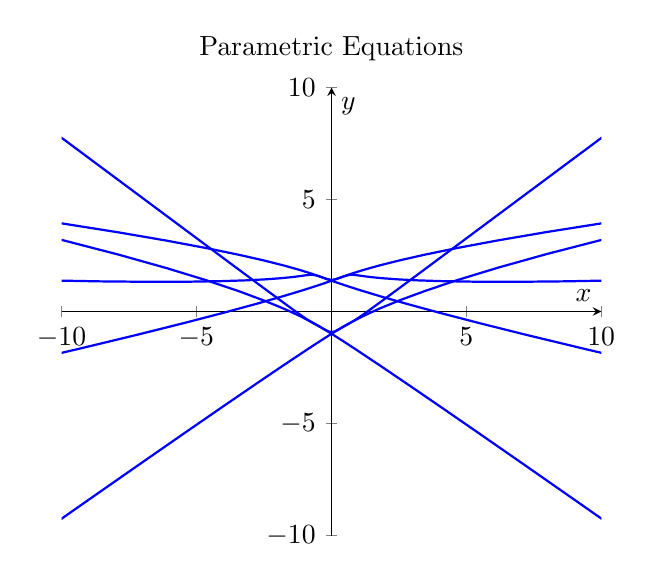
\begin{tikzpicture}
\begin{axis}[
    domain=-10:10,
    samples=100,
    xmin=-10, xmax=10,
    ymin=-10, ymax=10,
    axis lines=center,
    xlabel=$x$, ylabel=$y$,
    title={Parametric Equations}]
\addplot[blue, thick, domain=-10:10] (
{- 1.732051 + 1.000000*x - 0.921539*x^2 + 0.614359*x^3},{nan + nan*x + nan*x^2 + nan*x^3});
\addplot[blue, thick, domain=-10:10] (
{- 1.039230 + 1.000000*x - 0.921539*x^2 + 0.614359*x^3},{- 0.244143 - 0.826981*x + 0.871841*x^2 - 0.539711*x^3});
\addplot[blue, thick, domain=-10:10] (
{- 0.346410 + 1.000000*x - 0.921539*x^2 + 0.614359*x^3},{- 0.738993 - 0.702431*x + 0.702431*x^2 - 0.000000*x^3});
\addplot[blue, thick, domain=-10:10] (
{0.346410 + 1.000000*x - 0.921539*x^2 + 0.614359*x^3},{- 0.738993 + 0.702431*x - 0.747291*x^2 + 0.539711*x^3});
\addplot[blue, thick, domain=-10:10] (
{1.039230 + 1.000000*x - 0.921539*x^2 + 0.614359*x^3},{nan + nan*x + nan*x^2 + nan*x^3});
\addplot[blue, thick, domain=-10:10] (
{- 1.732051 + 1.000000*x - 0.921539*x^2 + 0.614359*x^3},{nan + nan*x + nan*x^2 + nan*x^3});
\addplot[blue, thick, domain=-10:10] (
{- 1.039230 + 1.000000*x - 0.921539*x^2 + 0.614359*x^3},{1.603378 + 0.173019*x - 0.154662*x^2 - 0.097987*x^3});
\addplot[blue, thick, domain=-10:10] (
{- 0.346410 + 1.000000*x - 0.921539*x^2 + 0.614359*x^3},{1.523748 - 0.430265*x + 0.430265*x^2});
\addplot[blue, thick, domain=-10:10] (
{0.346410 + 1.000000*x - 0.921539*x^2 + 0.614359*x^3},{1.523748 + 0.430265*x - 0.448622*x^2 + 0.097987*x^3});
\addplot[blue, thick, domain=-10:10] (
{1.039230 + 1.000000*x - 0.921539*x^2 + 0.614359*x^3},{nan + nan*x + nan*x^2 + nan*x^3});
\end{axis}
\end{tikzpicture}
\end{document}
